  \begin{minipage}{0.45\linewidth}
    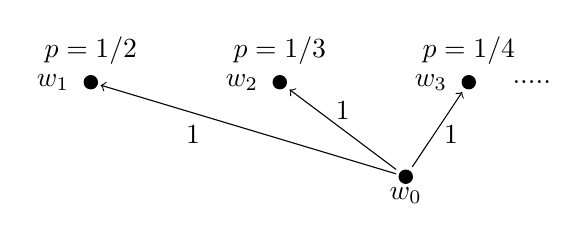
\begin{tikzpicture}[scale=0.8]
      % WORLDS  
      % w0
      \draw[fill] (0,-0.5) circle (3pt)
      +(0,-0)   node (w0)  {}  % used to label the circle 
      +(0,-0.3) node  {$w_0$}
      ;
      
      % w1 
      \draw[fill]  (-5,1) circle (3pt)
      +(0,0)   node (w1)  {}  % used to label the circle 
      +(-0.6,0)  node  {$w_1$} 
      +(0,0.5) node  {$p=1/2$}
      ;
      
      % w2
      \draw[fill] (-2,1) circle (3pt)
      +(0,0)   node (w2)  {}  % used to label the circle 
      +(-0.6,0) node{$w_2$}
      +(0,0.5) node{$p=1/3$}
      ;
      
      % w3
      \draw[fill] (1,1) circle (3pt)
      +(0,0)   node (w3)  {}  % used to label the circle 
      +(-0.6,0) node{$w_3$}
      +(0,0.5) node{$p=1/4$}
      ;
      
      % DOTS
      
      \draw[fill] (2,1) node{.....}  ; 
      
      % ARROWS
      \draw[->] (w0) -- (w1) node[midway,above, xshift=-2em,yshift=-2ex] {1};
      \draw[->] (w0) -- (w2) node[midway, above] {1}  ;
      \draw[->] (w0) -- (w3) node[midway, above, xshift=0.5em,yshift=-2ex] {1} ;
    \end{tikzpicture}
  \end{minipage}
  % -----------------------------------------      
  \fcolorbox{black}{gray!10}{
    \begin{minipage}{18em}\small
      \[
      \begin{array}{l}
        W=\{\,w_j~|~j\geq 0\,\}
        \\[1ex]
        R(w_0,w_0)=0
        \quad\quad\quad\hspace{1ex}
        e(w_0,p)=0
        \\[1ex]
        R(w_0,w_k)=1 \;\; k \geq 1
        \quad
        e(w_k,p) = \frac{1}{k+1}\;\; k\geq 1
      \end{array}
      \]
    \end{minipage}
  } % end box    
  % -----------------------------------------  
  $\small
    e(w_0,\Box p) \;=\; \inf_{j\geq 0}\{\,  R(w_0,w_j)\to e(w_j,p)  \,\}
    \;=\; \inf\{\;
    \overbrace{0\to 0}^1,\;\overbrace{1 \to (1/2)}^{1/2}, \; \overbrace{1 \to (1/3)}^{1/3}, \; \overbrace{1 \to (1/4)}^{1/4},  \,\dots  \;\}\;=\;0
    $

%%% Local Variables: 
%%% mode: latex
%%% TeX-master: "goedelModalLogicWitnessNonCrisp"
%%% End: 
